\chapter{ผลการทดลอง}

\section{การทำนายกลุ่มของโปรไฟล์}

\label{chapter:result}
ในส่วนนี้เรานำเสนอการทดลองเชิงประจักษ์ที่เน้นการประเมินคุณของการแนะนำงาน โดยการทดลองนี้เราได้มีข้อมูลโปลไฟล์ผู้เชี่ยวชาญจาก Linkedin จำนวน 417 ตัวอย่าง และตำแหน่งงานจาก Indeex จำนวน 4,748 ตำอย่าง, ทั้งโปรไฟล์และตำแหน่งงานเนื่องจากเฟิลด์ไอทีที่กว้างขวางโปรไฟล์จึงมีความแตกต่างกันบ้างเล็กน้อยในแต่ละกลุ่มโปรไฟล์ จากภาพด้านล่างแสดงการกระจายของฟิล์ดย่อยภายในของโปรไฟล์ 417 รายการซึ่งแสดงให้เห็นถึงจำนวนนักพัฒนาที่มีเป็นจำนวนมาก
\newline
\begin{figure}[!h]
  \centering
  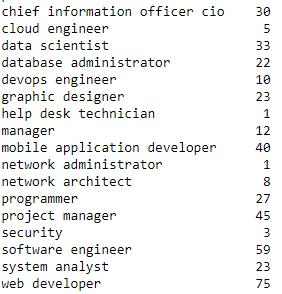
\includegraphics[width=0.5\textwidth]{profile_group.jpg}  
  \caption{การแยกกลุ่มของโปรไฟล์}
  \label{Fig:result-profile-group}
\end{figure}

ในการประเมินพวกเราได้ใช้ระบบแนะนำสร้างทำนายข้อมูลตำแหน่งงานสำหรับทดสอบ โดยใช้โมเดลที่ผ่านการเทรนมาแล้วได้โดยข้อมูลทดสอบนั้นเป็นข้อมูลรายละเอียดงานที่แบ่งมาจากส่วนเทรนจำนวน 33\% หรือ 1,567 ตัวอย่าง โดยจากรายงานการจำแนกประเภทเราจะเห็นว่าในกลุ่มตำแหน่งงานที่มีความคลุมเครือและใกล้เคียงกันเช่น 'web developer' และ 'software engineer' มีผลความแม่นยำที่น้อยเมื่อเทียบกับกลุ่มอื่น ๆ 

\begin{figure}[!h]
  \centering
  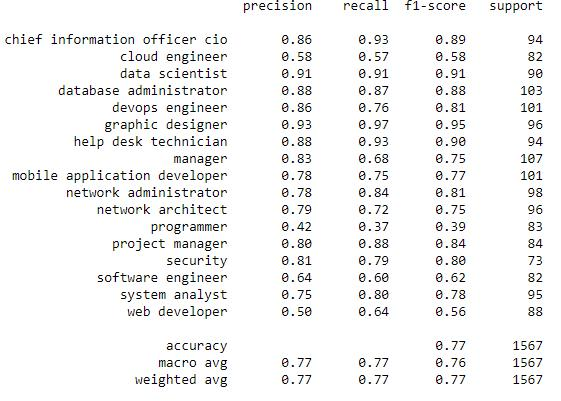
\includegraphics[width=0.95\textwidth]{classification_report.jpg}  
  \caption{รายงานการจำแนกประเภท}
  \label{Fig:result-classify-report}
\end{figure}

\newpage
ซึ่งจากการวิเคราะห์เราคาดว่าเกิดจากการใช้คำสำคัญ (keyword) ของโปรไฟล์ที่ดึงข้อมูลมาจาก linkedin โดยโปรไฟล์เหล่านี้มักใส่ทักษะวิชาชีพครอบคลุมในส่วนของการพัฒนาหรืออีกนัยคือ นักพัฒนาส่วนใหญ่เป็น full-stack ที่สามารถทำได้หลายตำแหน่งงาน แต่เนื่องจากตำแหน่งงานที่ทำในปัจจุบันของโปรไฟล์เหล่านั้นสามารถตั้งได้แค่ตำแหน่งเดียว ทำให้เกิดความคลาดเคลื่อนในการทำนาย
ทั้งนี้เมื่อเราทำการพล็อตการฟ confusion matrix เราจะเห็นถึงความผิดพลาดในการทำนายของตำแหน่ง 'software engineer' 'devops engineer' และ web developer เป็นจำนวนหนึ่งส่งผลให้ค่าความแม่นยำรวมเหลือแค่ 77\% ซึ่งทางเราถือว่าเกือบพอใช้ได้

\begin{figure}[!h]
  \centering
  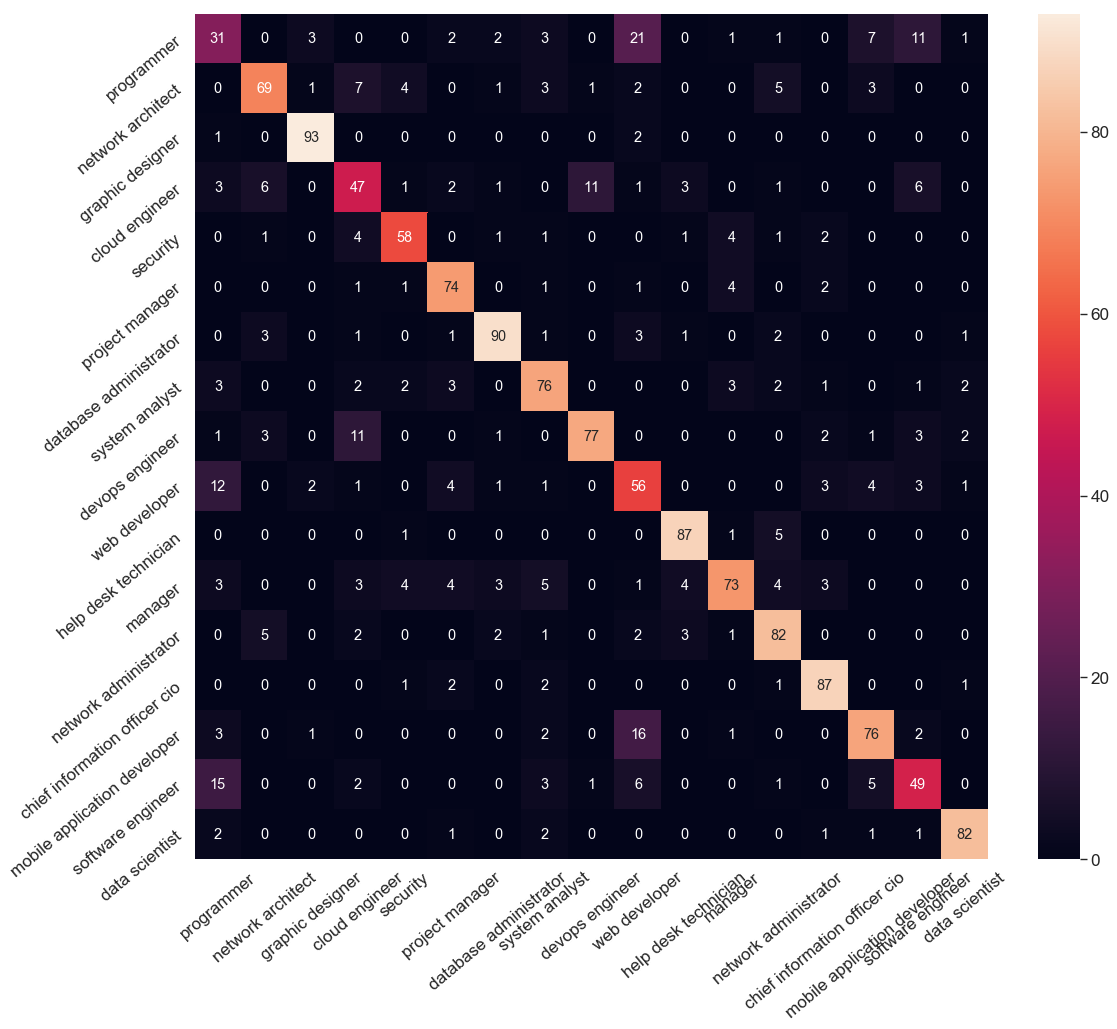
\includegraphics[width=1\textwidth]{confusion_matrix.png}  
  \caption{ตาราง confusion matrix}
  \label{Fig:result-classify-report}
\end{figure}

\newpage
\section{การจับคู่งานกับโปรไฟล์}
เราทำการแบ่งกลุ่มของโปรไฟล์ออกเป็นกลุ่มย่อย ๆ เนื่องจากในขั้นตอนการจับคู่งานกับโปรไฟล์โดยเทคนิคการหาระยะทางโคไซน์ (cosine distance) นั้นจำเป็นต้องใช้ทรัพย์ยากรเครื่องที่ประมวลผลเป็นจำนวนมาก การแบ่งกลุ่มออกเป็นกลุ่มย่อย ๆ จะช่วยแบ่งเบาภาระของการประมวลผลเพื่อหาตำแหน่งงานที่เหมาะสมกับโปรไฟล์ยูสเซอร์มากที่สุด

ผลลัพธ์การแนะนำตำแหน่งงานโดยการหาความสอดคล้องระหว่างโปรไฟล์ยูสเซอร์และงานในกลุ่ม เรายกตัวอย่างยูสเซอร์คนหนึ่งซึ่งเป็น senior software engineer ทำงานอยู่ agoda เพื่อเป็นตัวอย่างผลลัพธ์การแนะนำตำแหน่งงาน


\begin{figure}[!h]
  \centering
  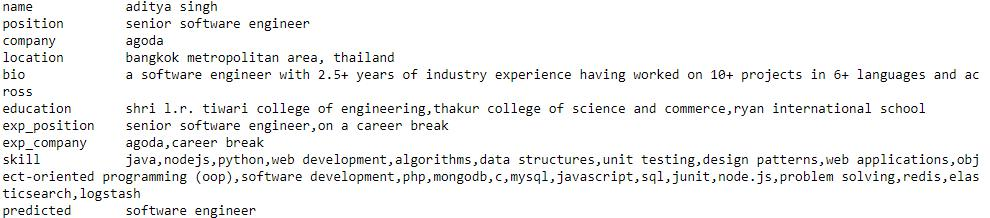
\includegraphics[width=1\textwidth]{user_example.jpg}  
  \caption{ตัวอย่างข้อมูลยูสเซอร์ในการแนะนำตำแหน่งงาน}
  \label{Fig:result-classify-report}
\end{figure}

\newpage

โดยเราทำการหา similarity distance ของตำแหน่งงานที่สอดคล้องกับโปรไฟล์นี้มากที่สุด 10 อันแรกจะได้ผลลัพธ์ตามนี้


\begin{figure}[!h]
  \centering
  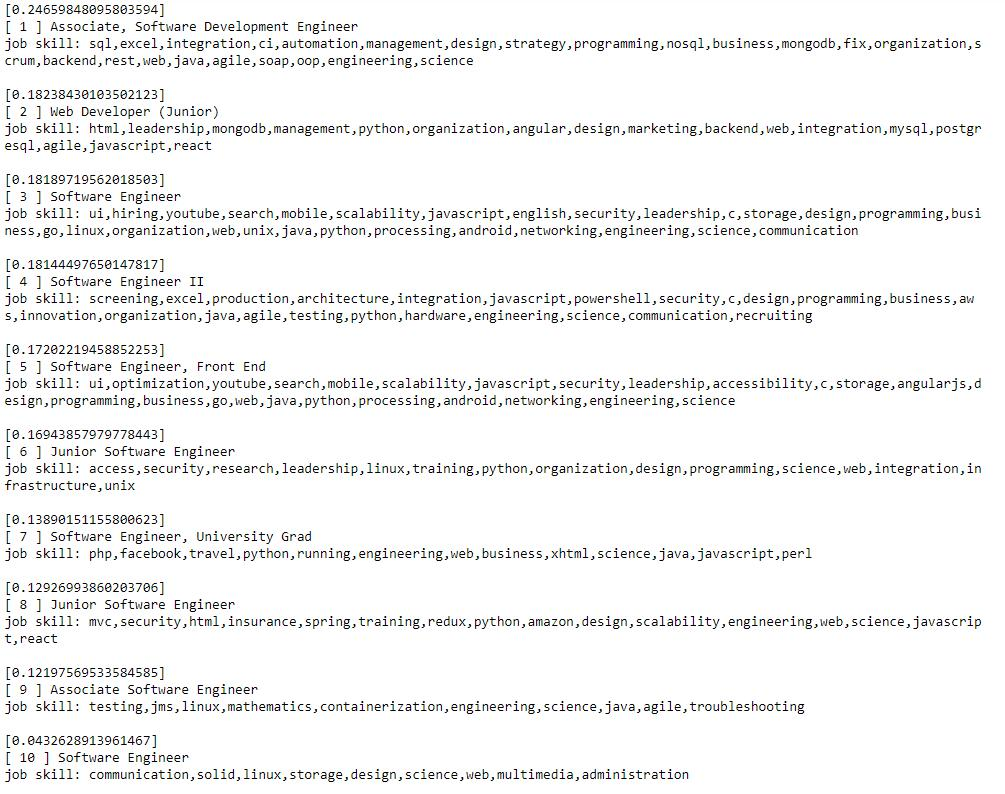
\includegraphics[width=1\textwidth]{recommend_result.jpg}  
  \caption{ผลการแนะนำตำแหน่งงานที่สอดคล้องกับยูสเซอร์มากที่สุด 10 อันแรก}
  \label{Fig:result-classify-report}
\end{figure}